%\documentclass[9pt, compress, xcolor=table, draft]{beamer}
\documentclass[9pt, compress, xcolor=table]{beamer}


\usetheme{m}

\usepackage{amsmath,amssymb,amsthm}
\usepackage{latexsym}
\usepackage{booktabs}
\usepackage[scale=2]{ccicons}
\usepackage{minted}
\usepackage[english, russian]{babel}
\usepackage{graphicx}
\usepackage{xcolor}
\usepackage{euscript}
% \DeclareMathOperator{\arctg}{arctg}
\usepackage{tabu} % https://ru.sharelatex.com/learn/Tables
\DeclareGraphicsExtensions{.pdf,.jpg,.png}
\graphicspath{{../images/}{./images/}}

\colorlet{Mycolor1}{green!50!blue!50!}
\DeclareMathOperator{\Ima}{Im}
\usemintedstyle{trac}

\title{Физические принципы оптической микроскопии сверхвысокого разрешения}
\subtitle{осенний семестр, 2015}
\author{ассистент, к.ф.-м.н. Шутова О.А.}
\institute{МГУ им. М.В. Ломоносова, физический факультет}

\begin{document}

\maketitle

\plain{}{Лекция 7. Явления в области полного внутреннего отражения}

\begin{frame}{Идея лекции}

Ранее мы описали явление полного внутреннего отражения (\textcolor{red!50!black}{TIR, total internal reflection}) и сказали, что это явление представляет собой наиболее простой и естественный способ создания неоднородной (эванесцентной) волны. 

Мы также ввели понятие нарушенного полного внутреннего отражения (\textcolor{red!50!black}{FTIR, frustrated total internal reflection}) и обозначили его важную роль в процессе преобразования неоднородной волны в распространяющуюся к детектору, находящемуся в дальней зоне.

Сегодня мы рассмотрим являние в схеме оcлабленного полного внутренего отражения (\textcolor{red!50!black}{ATIR, attenuated total internal reflection} и биосенсоры на основе этой схемы). Так как коэффициенты Френеля в точке ПВО имеют особенность в своем поведении, область вблизи ПВО обладает высокой чувствительностью к свойствам среды. Один из примеров, интересных в этом плане,~--- сдвиг пространственно-ограниченных пучков при отражении от поверхности, т.н. \textcolor{red!50!black}{сдвиг Гуса-Хенхен}, впервые описанный И. Ньютоном в трактате \textbf{Оптика} и измеренный F.~Goos и H. H\"{a}nchen в 1947.

\end{frame}

\begin{frame}{Сдвиг Гуса-Хенхен}
\begin{center}
\begin{equation*}
R(k_x)=|R(k_x)|e^{\imath \phi(k_x)}\quad\text{коэффициент отражения Френеля}
\end{equation*}

В области ПВО:$|R(k_x)|= 1$ и, если фаза меняется не очень быстро,
\begin{equation*}
\phi(k_x) = \phi(k_x=k_{x0})+\beta\frac{\partial \phi(k_x)}{\partial k_x}(k_x=k_{x0})+\beta^2\frac{\partial^2 \phi(k_x)}{\partial k_x^2}(k_x=k_{x0})+...
\end{equation*}

для амплитуды отраженного пучка можно получить:
\begin{equation*}
|u_R(x,l)|=|R(k_{x0})||u_R(x+\delta,l)|,
\end{equation*}

где $\delta =\frac{\partial \phi(k_x)}{\partial k_x}(k_x=k_{x0})=-\frac{1}{k \cos \theta}\frac{\partial \phi}{\partial \theta}$

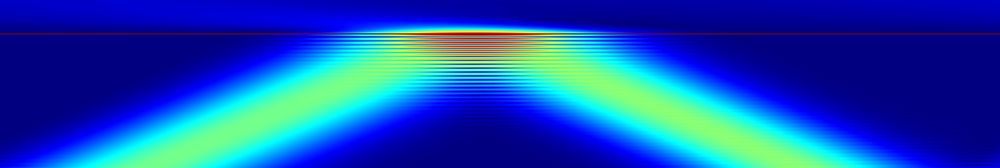
\includegraphics[width=\textwidth]{gh0_small}
\end{center}

{\small М.Б. Виноградова, О.В. Руденко, А.П. Сухоруков. Теория волн. М.: Наука, 1990.  Гл.7, пар. 7 Отражение ограниченных волновых пучков, стр. 273.}
\end{frame}

\begin{frame}{Дефазировка в коэффициентах Френеля}

\begin{center}
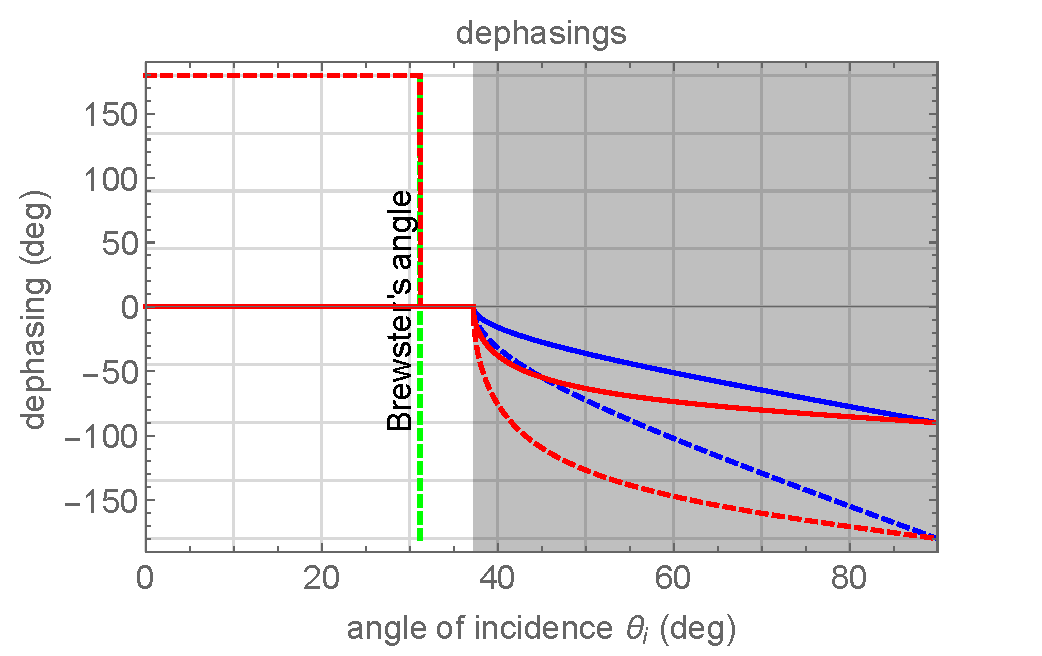
\includegraphics[width=0.8\textwidth]{fresnel}
\end{center}

\begin{equation*}
R_{\perp} =\frac{n_i\cos\theta_i-n_t\cos\theta_t}{n_i\cos\theta_i+n_t\cos\theta_t}=|R_{\perp}|\exp(\imath\phi_{\perp})
\end{equation*}

\begin{equation*}
R_{||} =\frac{n_t\cos\theta_i-n_i\cos\theta_t}{n_i\cos\theta_t+n_t\cos\theta_i}=|R_{||}|\exp(\imath\phi_{||})
\end{equation*}

\end{frame}

\begin{frame}{Вычисление сдвига для разных поляризаций}
\begin{columns}[c]
\column{6.3cm}
\begin{center}
Фаза коэффициента отражения Френеля для s-поляризации
\begin{equation*}
\phi_{\perp} = -2\arctg \sqrt{\left(\frac{k_x^2-k^2 n^2}{k^2-k^2_x}\right)}
\end{equation*}

\begin{equation*}
\Delta_{\perp} = -\frac{\lambda}{\pi}\frac{\tg \theta}{\sqrt{(\sin^2 \theta - n^2)}}
\end{equation*}

\end{center}
\column{6.3cm}
\begin{center}
Фаза коэффициента отражения Френеля для p-поляризации
\begin{equation*}
\phi_{||} = -2\arctg \sqrt{\left(\frac{k_x^2-k^2 n^2}{n^2(k^2-k^2_x)}\right)}
\end{equation*}

\begin{equation*}
\Delta_{||} = \frac{n^2}{\sin^2\theta(1+n^2)-n^2}\Delta_{\perp}
\end{equation*}
\end{center}
\end{columns}
\begin{itemize}
\item Сдвиг Гуса-Хенхен можно рассматривать как чисто интерференционное явление
\item Сдвиг Гуса-Хенхен можно интерпретировать как перенос энергии ЭМ излучения вдоль границы эванесцентным полем 
\item Если учесть вторую производную, можно получить также сдвиг вдоль направления распространения
\item Можно рассматривать сдвиг как задержку прохождения света, связанную с процессами рассеяния
\item Масштаб величины сдвига не превышает длину волны света
\end{itemize}
\end{frame}

\begin{frame}{Зависимость величины сдвига от угла}
\begin{center}
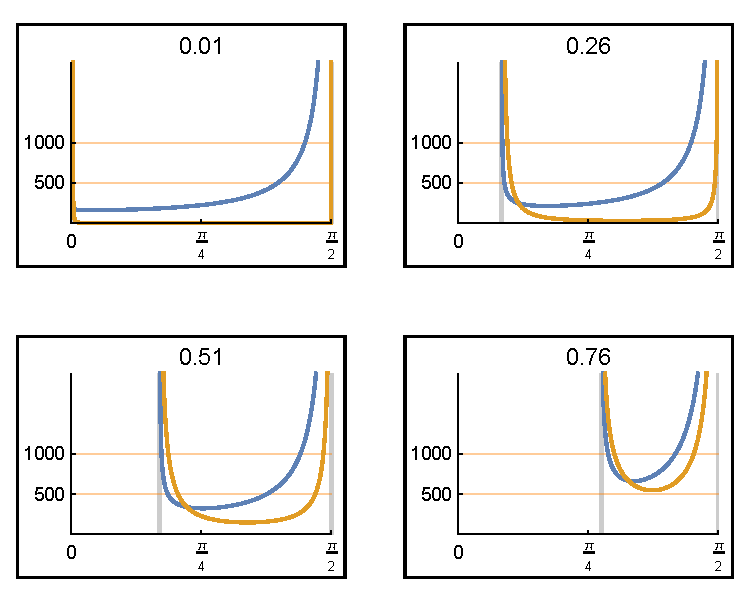
\includegraphics[width=0.8\textwidth]{gh}

над графиком показана величина относительного показателя преломления $n=\sqrt{\epsilon_1/\epsilon_2}$
\end{center}
\end{frame}
\begin{frame}{Зависимость отношения p/s поляризаций от угла}
\begin{center}
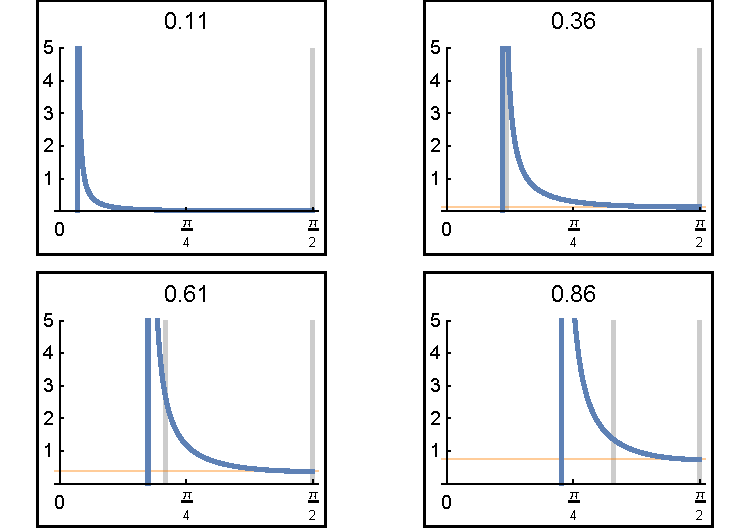
\includegraphics[width=0.8\textwidth]{gh1}

над графиком показана величина относительного показателя преломления $n=\sqrt{\epsilon_1/\epsilon_2}$
\end{center}
\end{frame}


\begin{frame}{Сдвиг Гуса-Хэнхен}
\begin{columns}[c]
\column{1.8in}

\begin{equation*}
\tilde{n} = \frac{\sqrt{\epsilon_1 \mu_1}}{\sqrt{\epsilon_2 \mu_2}}
\end{equation*}
\begin{equation*}
\left[1-\tilde{n^2} \sin^2 \theta_1\right] = 0
\end{equation*}
\begin{equation*}
\theta_c = \arcsin [1/ \tilde{n}]
\end{equation*}
\begin{equation*}
\gamma = k_2 \sqrt{\tilde{n}^2 \sin^2 \theta_1 - 1}
\end{equation*}

\begin{center}
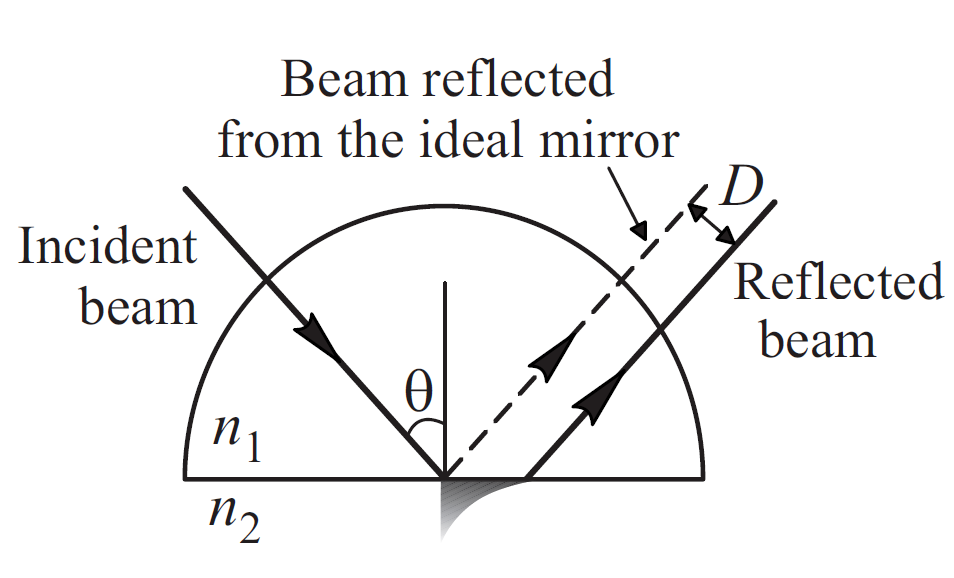
\includegraphics[scale=0.14]{gh01}
\end{center}


\column{2.8in} Сдвиг Гуса-Хэнхен фазы прошедшей и отраженной волн относительно угла падения (1943
г.)
\begin{center}
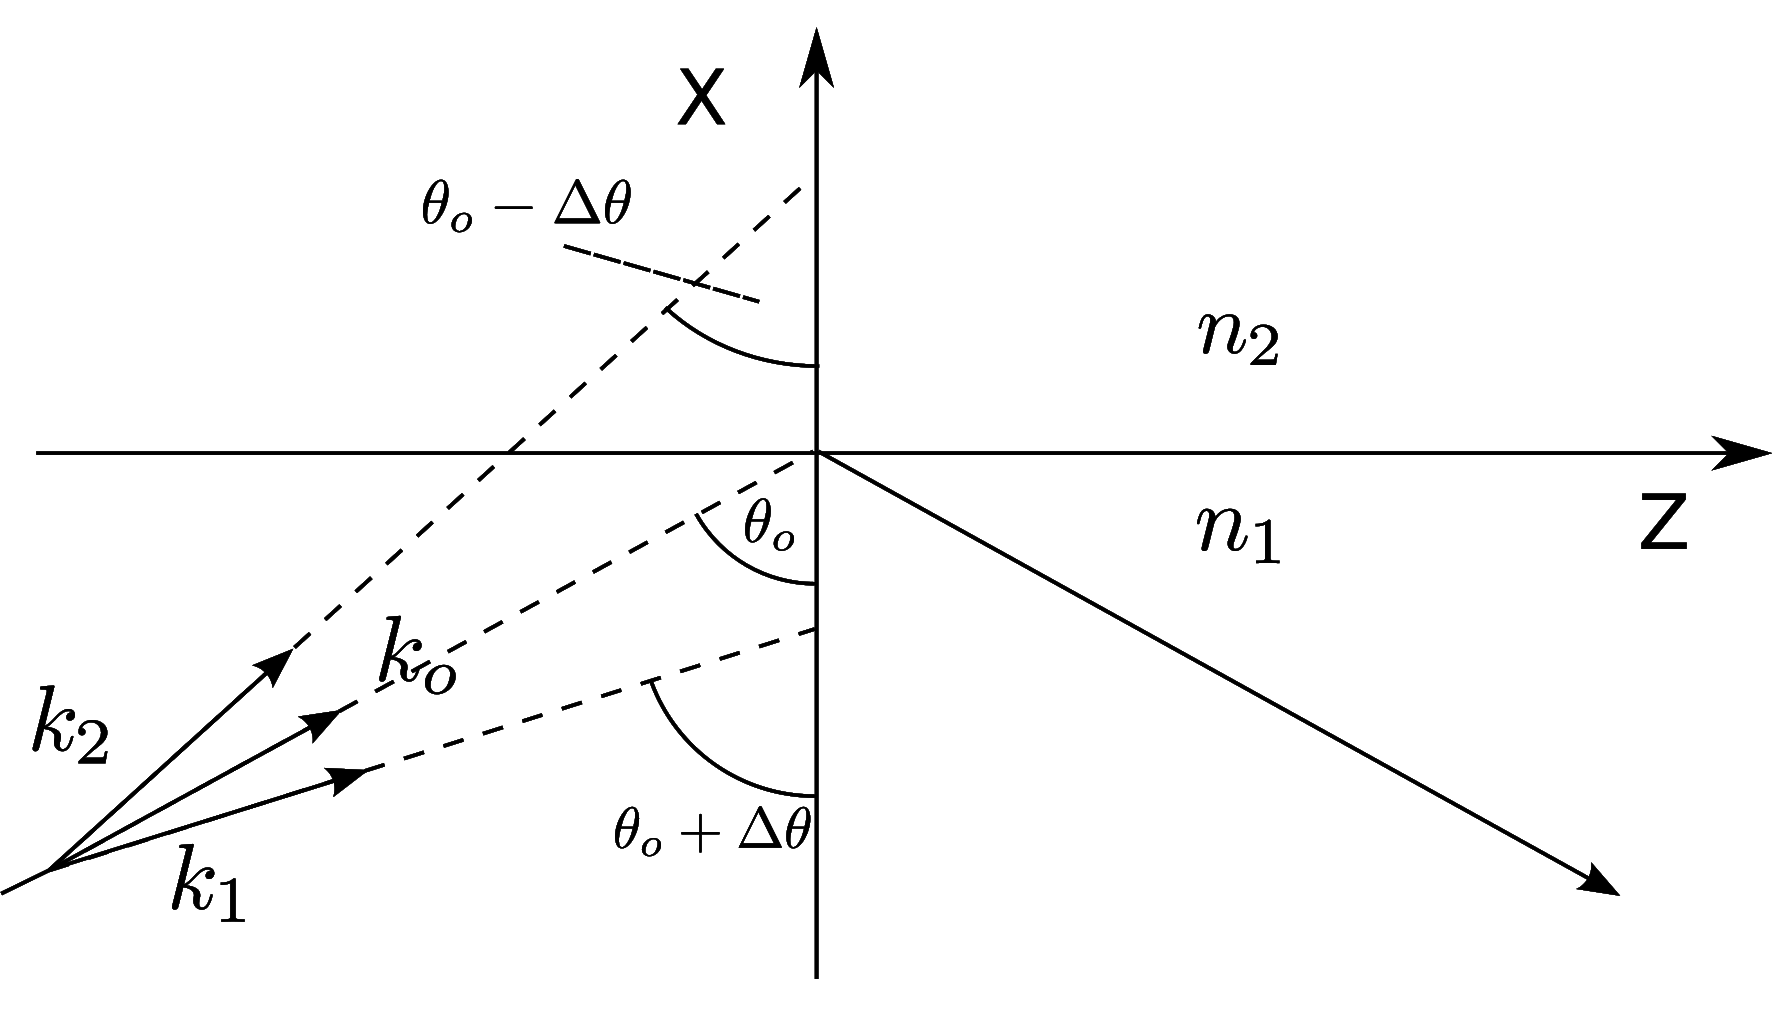
\includegraphics[scale=0.12]{fig2_12}
\end{center}

\end{columns}

Для величины поперечного сдвига (сдвига в направлении, перпендикулярном см. статью M/ McGuirk, С.K. Carniglia An angular spectrum representation approach too the Goos-H\"{a}nchen shift)

\end{frame}

\begin{frame}{Электродинамическая интерпретация сдвига Гуса-Хенхен}
\begin{columns}[c]
\column{6.5cm}
\begin{equation*}
E_{2y} = {\vec E}_2(x,z,t) \exp\left[ \imath ( k_{1x} x - \omega_0 t )\right],
\end{equation*}

\begin{equation*}
\left| \frac{\partial^2 {\vec E}_2}{\partial x^2} \right| \ll |k_{1x}| \left| \frac{\partial {\vec E}_2}{\partial x} \right|, \quad  \left| \frac{\partial^2 {\vec E}_2}{\partial t^2} \right| \ll \omega_0 \left| \frac{\partial {\vec E}_2}{\partial t} \right|
\end{equation*}

\begin{equation*}
\lim_{z \to \infty} {\vec E}_2= 0.
\end{equation*}
\column{6.5cm}
\begin{equation*}
E_{1y} = {\vec E}_1(x,z,t) \exp\left[ \imath ( k_{1x} x + k_{1z}z -\omega_0 t )\right],
\end{equation*}

\begin{equation*}
\left| \frac{\partial^2 {\vec E}_1}{\partial x^2} \right| \ll |k_{1x}| \left| \frac{\partial {\vec E}_1}{\partial x} \right|, \quad  \left| \frac{\partial^2 {\vec E}_1}{\partial z^2} \right| \ll k_{1z} \left| \frac{\partial {\vec E}_1}{\partial z} \right|, 
\end{equation*}

\begin{equation*}
\left| \frac{\partial^2 {\vec E}_1}{\partial t^2} \right| \ll \omega_0 \left| \frac{\partial {\vec E}_1}{\partial t} \right|.
\end{equation*}

\begin{equation*}
\lim_{|x| \to \infty} {\vec E}_1= \lim_{|z| \to \infty} {\vec E}_1 = 0,
\end{equation*}

\begin{equation*}
\lim_{|t| \to \infty} {\vec E}_1 =  0.
\end{equation*}
\end{columns}
\begin{equation*}
\boxed{2\imath \frac{\omega_0 n_2^2}{c^2} \frac{\partial {\vec E}_2}{\partial t} + 2\imath k _{1x} \frac{\partial {\vec E}_2}{\partial x} +  \frac{\partial^2 {\vec E}_2}{\partial z^2} + \left( k_2^2 - k_{1x}^2 \right)  {\vec E}_2 = 0}
\end{equation*}

\end{frame}

%%================================================================

\begin{frame}{Закон сохранения энергии}

\begin{equation*}
I_z(0) = \frac{c}{8\pi k_0} \int_{-\infty}^{\infty}  \left[ \frac{1}{2\imath} \left( \frac{\partial  {\vec E}_2}{\partial z}{\vec E}_2^* -  \frac{\partial  {\vec E}_2^*}{\partial z}{\vec E}_2 \right)  \right] dx, \quad z=0.
\end{equation*}

\begin{equation*}
w = \frac{\epsilon_2}{8\pi} |{\vec E}_2 |^2
\end{equation*}

\begin{equation*}
I_z(0) = \frac{\partial}{\partial t} \left( \int_0^{\infty} dz \int_{-\infty}^{\infty} w \, dx \right),
\end{equation*}
\begin{equation*}
k_z(x,\omega) = \imath \sqrt{ k_{1x}^2 - k_2^2 +2k_{1x}k_x - \frac{2\omega\omega_0\epsilon_2}{c^2} }, \quad \Im k_z >0,
\end{equation*}

\begin{equation*}
{\vec E}_2(x,y,z) = \iint_{-\infty}^{\infty} A_2(k_x,\omega) \exp\left[ \imath \left( k_xx + k_z(k_x,\omega)z - \omega t \right) \right]  dk_x d\omega.
\end{equation*}

\begin{equation*}
k_z \approx \imath \sqrt{k_{1x}^2-k_2^2} \left[ 1 + \frac{k_{1x}}{k_{1x}^2-k_2^2}k_x - \frac{\omega_0\epsilon_2}{c^2 (k_{1x}^2-k_2^2)}\omega \right].
\end{equation*}


\end{frame}


\begin{frame}{Линейная плотность потока энергии через границу $z=0$}

\begin{equation*}
I_z(0) = \frac{c}{8\pi k_0} \int_{-\infty}^{\infty} \left[ \frac{k_{1x}}{\sqrt{k_{1x}^2-k_2^2}} \frac{\partial |{\vec E}_2|^2}{\partial x} + \frac{\omega_0 \epsilon_2}{c^2 \sqrt{k_{1x}^2-k_2^2}} \frac{\partial |{\vec E}_2|^2}{\partial t}  \right] dx
\end{equation*}

\begin{equation*}
{\vec E}_2(x,0,t) = \frac{2k_{1z}}{k_{1z} + \imath \sqrt{k_{1x}^2-k_2^2}} {\vec E}_1(x,0,t), \quad (z=0)
\end{equation*}


\begin{multline}
I_z(0) = \frac{c k_{1z}^2}{2 \pi k_0 (k_1^2-k_2^2)} \times \\
\times \int_{-\infty}^{\infty} \left[ \frac{k_{1x}}{\sqrt{k_{1x}^2-k_2^2}} \frac{\partial |{\vec E}_1|^2}{\partial x} + \frac{\omega_0 \epsilon_2}{c^2 \sqrt{k_{1x}^2-k_2^2}} \frac{\partial |{\vec E}_1|^2}{\partial t} \right] dx
\end{multline}

\begin{equation*}
E_{2y} \, \text{и} \, H_{2x} = \frac{\imath}{k_0} \frac{\partial E_{2y}}{\partial z} = \frac{\imath}{k_0} \frac{\partial \vec E_2}{\partial z} \exp \left[ \imath (k_{1x}x - \omega t) \right]
\end{equation*}

Формула, описывающая поток энергии, связанный с формированием преломленной волны, соответствует коллективному механизму переноса энергии, где весь континуум фурье-компонент преломленной волны выступает как единое целое.

\end{frame}

\begin{frame}{Электродинамическая интерпретация сдвига Гуса-Хенхен}

Энергия переносится в отражающую среду для той части падающего пучка, где выполняется условие 
\[ 
k_{1x} \frac{\partial |\vec E_1|^2}{\partial x} > 0,
\]
и переносится из отражающей среды в исходную для той части падающего пучка, где выполняется условие  
\[ 
k_{1x} \frac{\partial |\vec E_1|^2}{\partial x} < 0.
\]

В силу ГУ $I_z(0) = 0$. Если с одной стороны падающего пучка некоторое количество энергии "<втекает"> в отражающую среду, то с другой стороны падающего пучка точно такое же количество энергии "<вытекает"> из этой среды, приводя к боковому сдвигу отраженного пучка, который и есть сдвиг Гуса-Хенхен.

\end{frame}


\begin{frame}{Качественное объяснение}
\begin{columns}[c]
\column{6.5cm}
\begin{center}
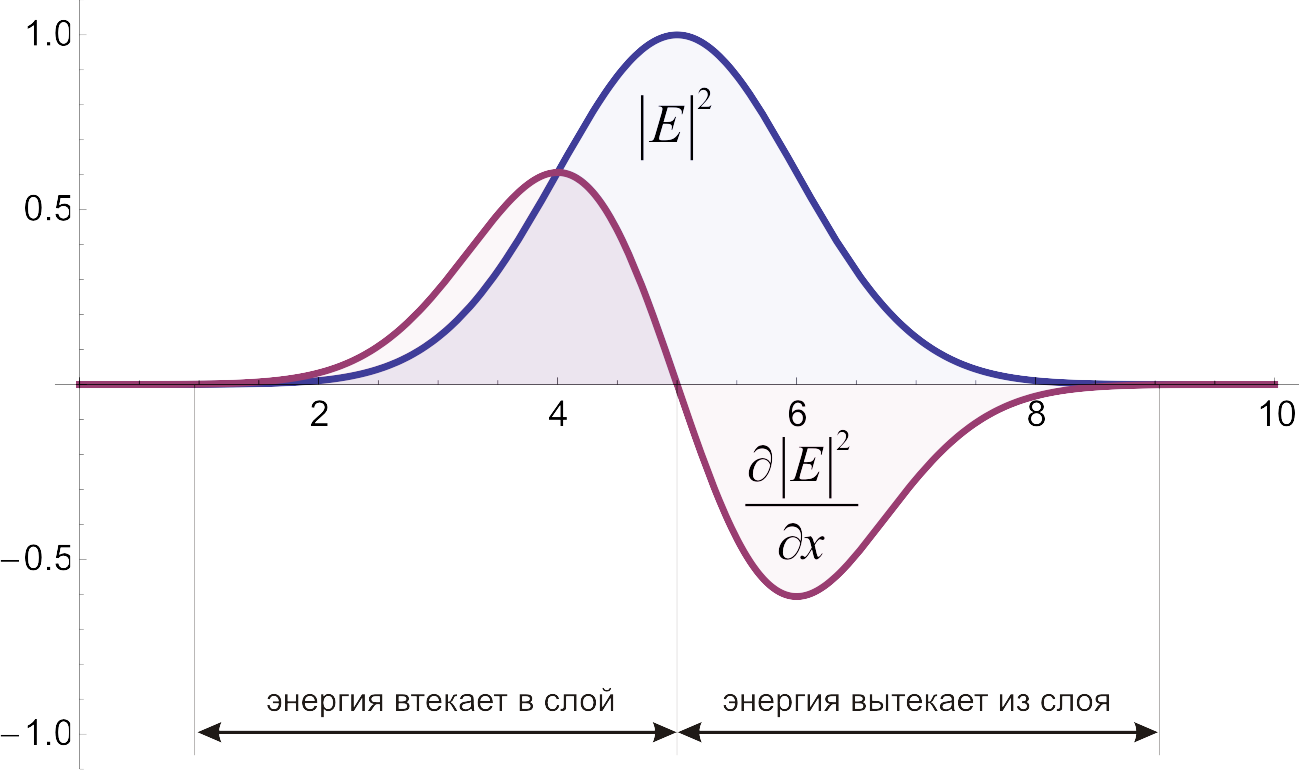
\includegraphics[width=0.9\textwidth]{Goos-Hanchen_effect_Gauss}
\end{center}
\column{6.5cm}
\begin{center}
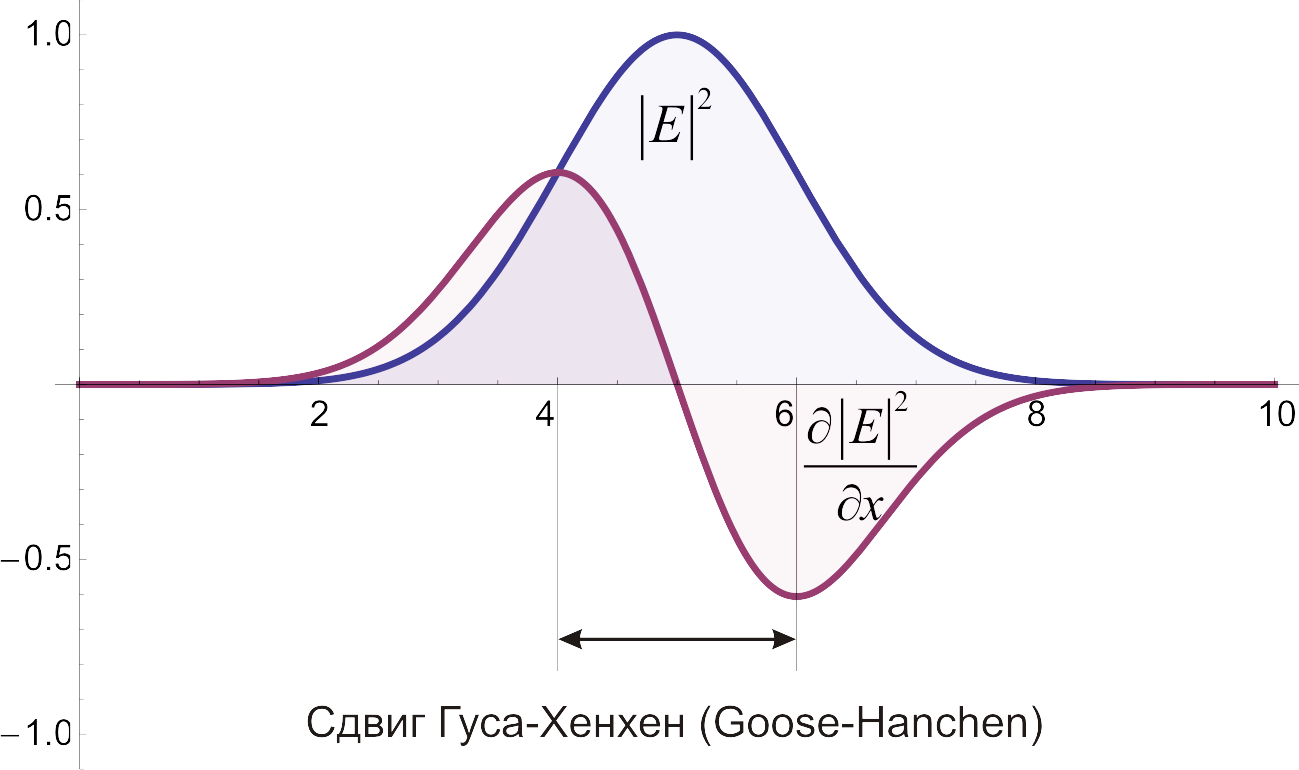
\includegraphics[width=0.9\textwidth]{Goos-Hanchen_effect_Gauss_shift}
\end{center}
\end{columns}
\end{frame}

\plain{}{Усиление сдвига Гуса-Хенхен и сенсорные устройства на его основе}

\begin{frame}{Сдвиг Гуса-Хенхен при возбуждении SPP}
\begin{columns}[c]
\column{6.3cm}
\begin{center}
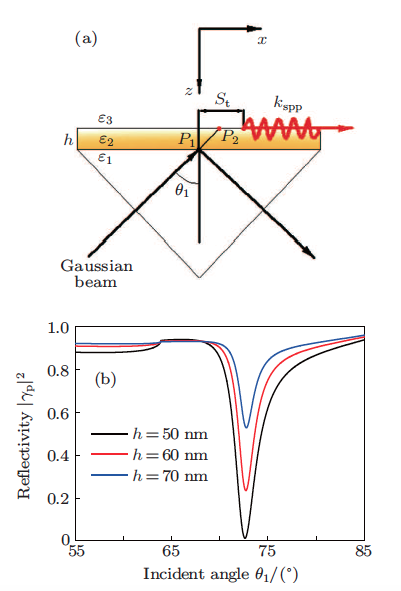
\includegraphics[width=0.8\textwidth]{gh15}
\end{center}
\column{6.3cm}
\begin{center}
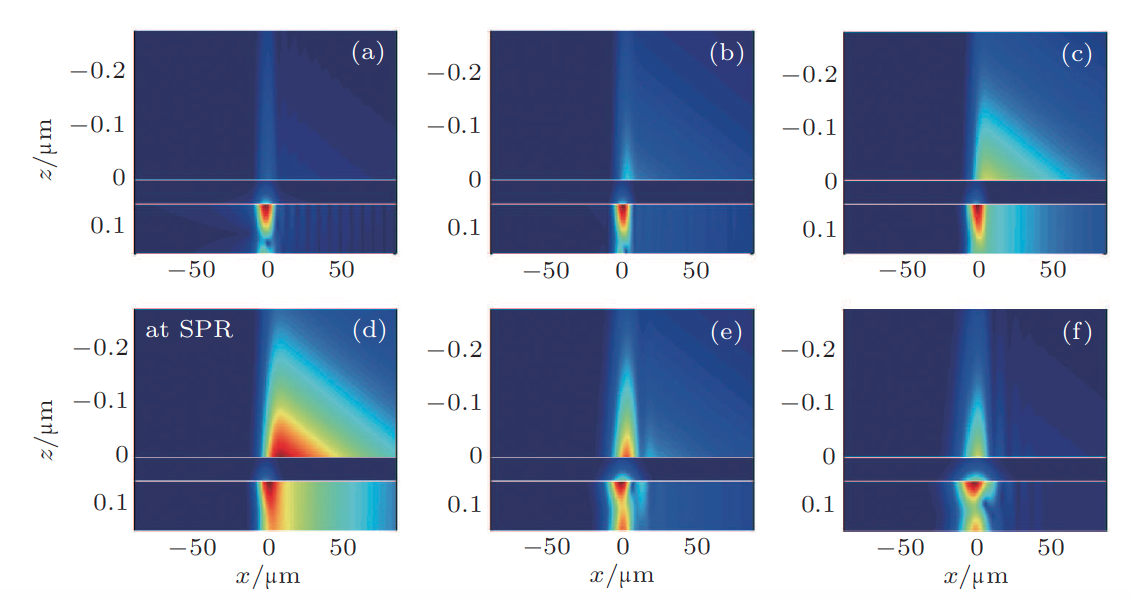
\includegraphics[width=0.9\textwidth]{gh8}

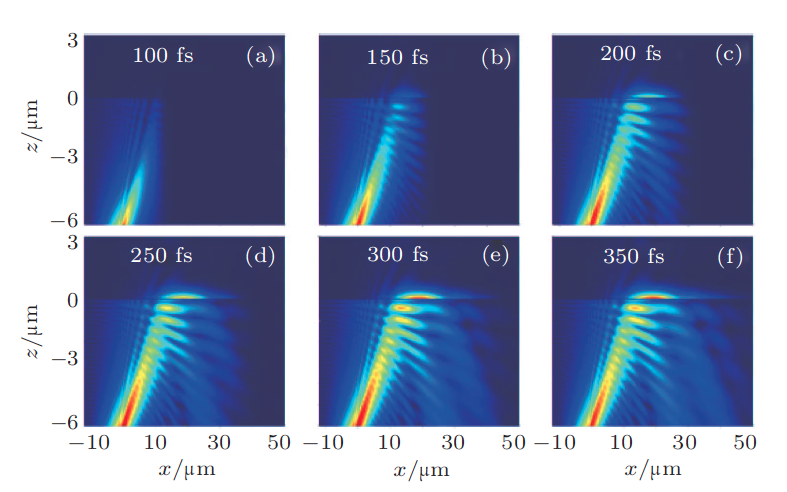
\includegraphics[width=0.9\textwidth]{gh10}
\end{center}

$\theta_{SPP}=72.68^{o}$

$\theta_{TIR}=65.6^{o}$
\end{columns}
Y.Yang et al. Chin. Phys. B, v.24, n.7, 2015.
\end{frame}

\begin{frame}{Сдвиг Гуса-Хенхен в условиях SPP}
\begin{center}
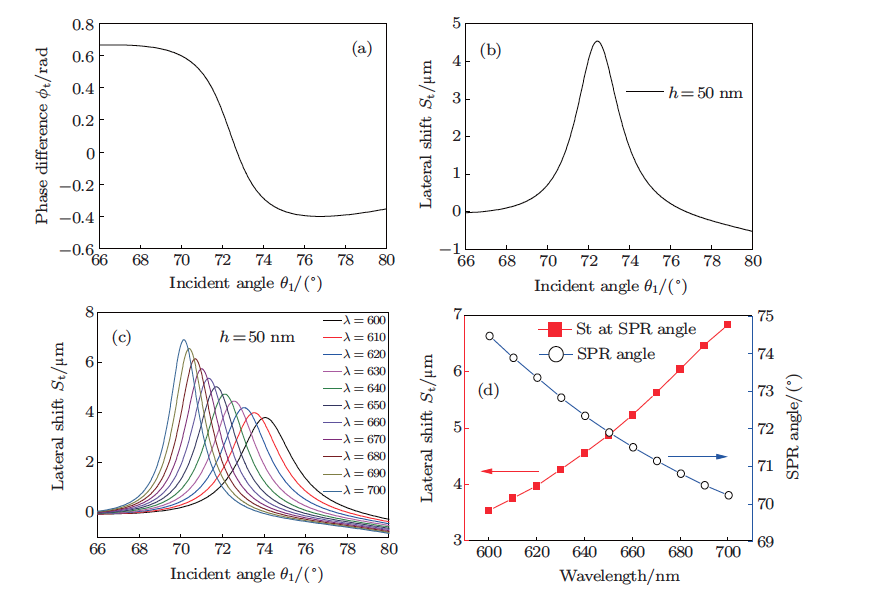
\includegraphics[width=\textwidth]{gh9}
\end{center}
\end{frame}

\begin{frame}{Поведение фазы коэффициента пропускания Френеля}

\begin{center}
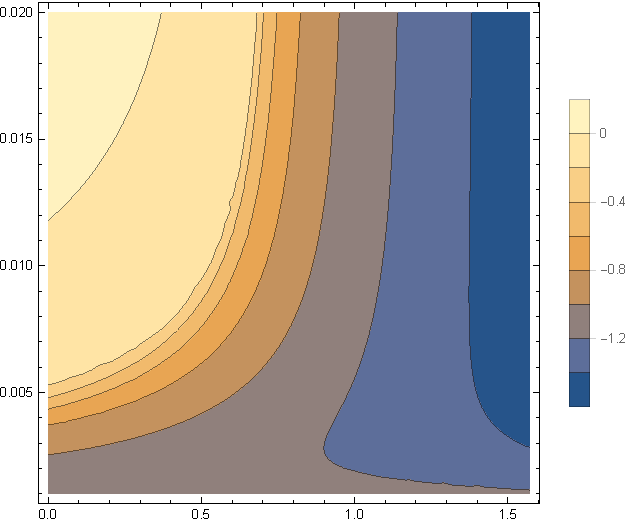
\includegraphics[width=0.6\textwidth]{phase}
\end{center}

\begin{equation*}
T(k_{||})=\frac{2\epsilon_2(\omega)\sqrt{\omega/c\sqrt{\epsilon_1}-k_{||}^2}}{\epsilon_2(\omega)\sqrt{\omega/c\sqrt{\epsilon_1}-k_{||}^2}+\epsilon_1\sqrt{\omega/c\sqrt{\epsilon_2(\omega)}-k_{||}^2}}\sqrt{\frac{\epsilon_1}{\epsilon_2(\omega)}}
\end{equation*}

где $k_{||}=k_1\sin[\theta]$

\end{frame}

\begin{frame}{Поверхностные сенсоры}

Поверхностные сенсоры появились в 1982 г. и к настоящему времени это уже стандартные приборы в области биохимических исследований. Вопрос состоит в повышении чувствительности этих приборов, чтобы уметь наблюдать сверхнизкие концентрации искомого вещества.

\vspace{0.5cm}

$\boxed{\text{Идея прибора: высокая чувствитиельность SPR к показателю преломления}}$

\vspace{0.5cm}

Измерять сдвиг Гуса-Хенхен - это замена более затратным методам модуляционных, интерференционных методик или эллипсометрии.

\vspace{0.5cm}

Рассмотрим работу группы L. Hesselink, Stanford University (Appl.Phys. Lett., 2006)


\end{frame}


\begin{frame}{Поверхностные сенсоры на основе свдига Гуса-Хенхен}
Усиление в схеме ATIR (с возбуждением поверхностного плазмона-поляритона)

\begin{columns}[c]
\column{2.8in}
\begin{center}
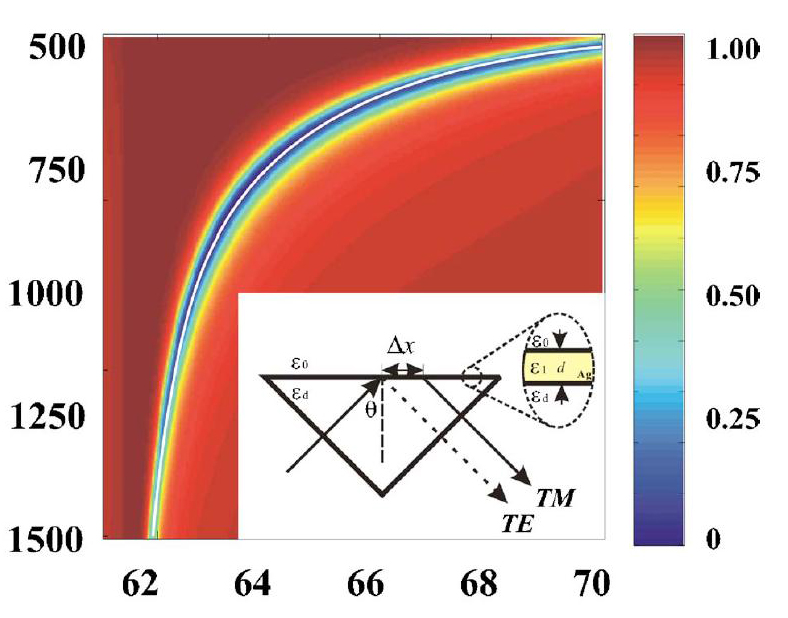
\includegraphics[scale=0.3]{gh5}
\end{center}
{\small Зависимость амплитуды отраженного света от угла падения и длины волны}

\column{1.8in}


Дисперсионное соотношение для поверхностного плазмон-поляритона

$k_x = k_0 \sqrt{\epsilon_m^{'} \epsilon_d / (\epsilon_m^{'}+ \epsilon_d) }$

где $\epsilon_d$ - диэлектрическая проницаемость диэлектрика (стекло); $\epsilon_m^{'}$ -
действительная часть диэлектрической проницаемости металла (золото)

\end{columns}
Толщина пленки золота на поверхности призмы 42 нм.
\end{frame}
\begin{frame}{Усиление сдвига Гуса-Хенхен при возбуждении SPP}

\begin{columns}[c]
\column{2.8in}
\begin{center}
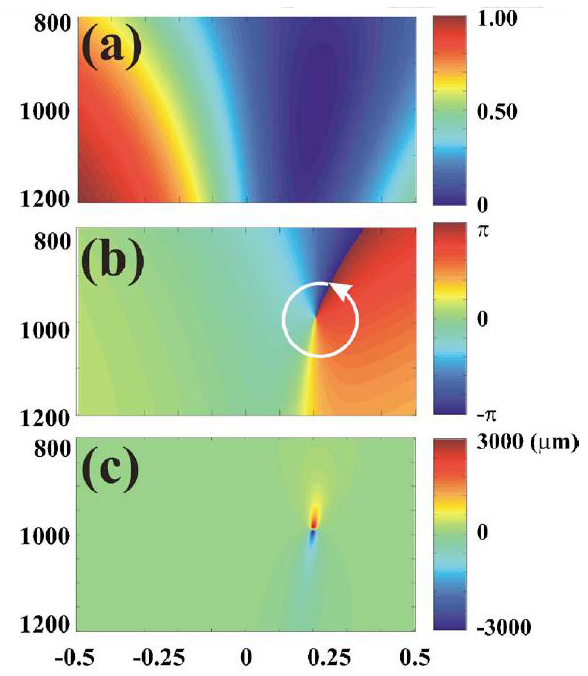
\includegraphics[width=0.8\textwidth]{gh6}
\end{center}

\column{1.8in}

Величина $\Delta x$ определяется из соображений непрерывности фазы:

$\Delta x = -\partial \Phi_R / \partial k_x$,

где $\Phi_R$ - фазовая задержка отраженной волны.

Рисунок:

(a) коэффициент отражения;

(b) фаза;

(c) сдвиг Гуса-Хенхен;
\end{columns}

\end{frame}


\begin{frame}{Схема эксперимента и результаты}
\begin{columns}[c]
\column{6.3cm}
\begin{center}
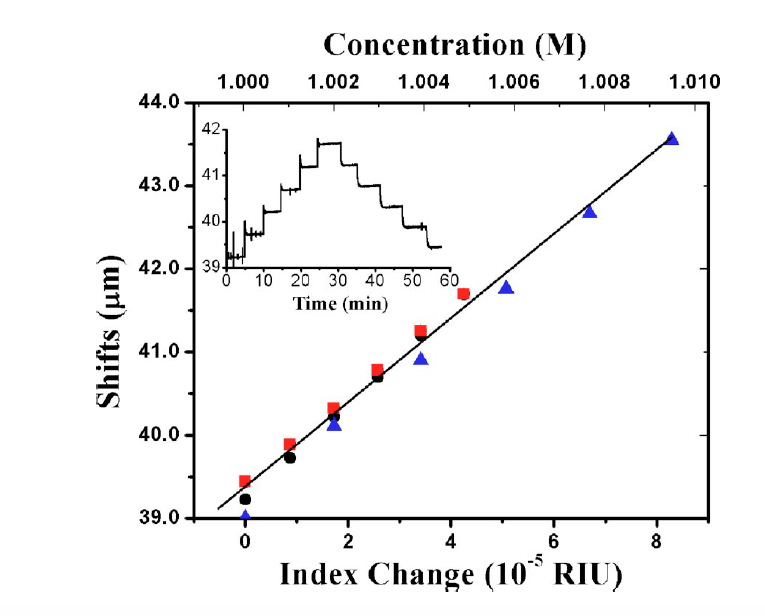
\includegraphics[width=0.9\textwidth]{gh12}
\end{center}
\column{6.3cm}
\begin{center}
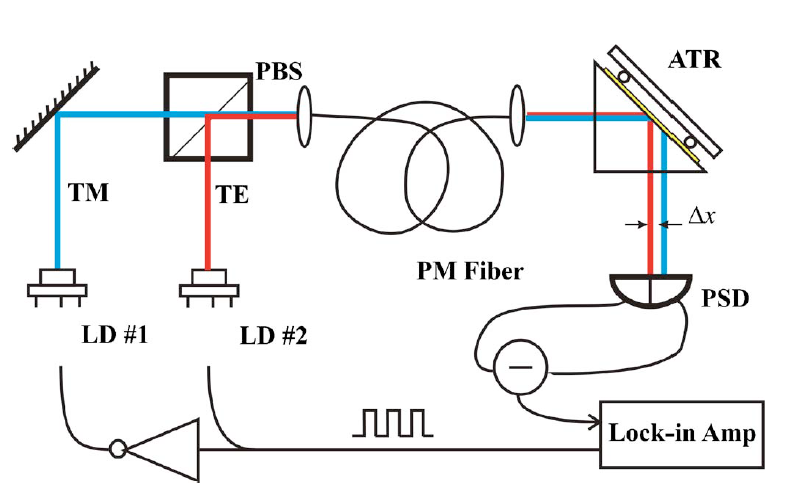
\includegraphics[width=0.9\textwidth]{gh13}
\end{center}
\end{columns}

RIU - reflective index units

Пространственное разрешение PSD - 20 нм. 

Разрешаемое изменение покаазателя преломления $4*10^{-7}$ RIU.

\end{frame}

\begin{frame}{Усиление сдвига Гуса-Хенхен на фотонном кристалле }
научная группа А.А. Федянина, МГУ
\begin{columns}[c]
\column{3in}
\begin{center}
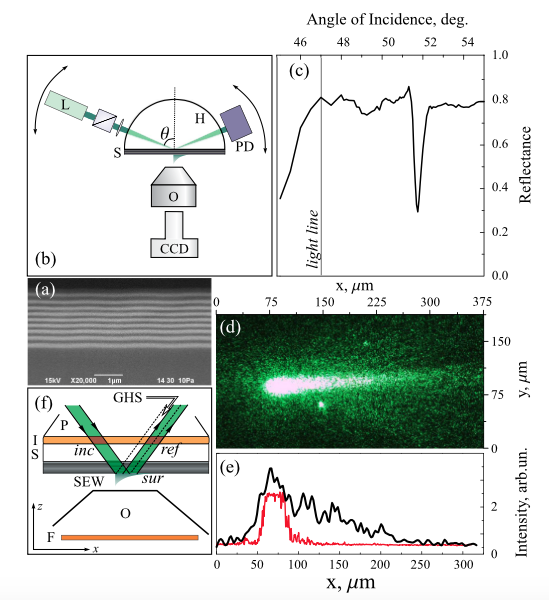
\includegraphics[width=0.9\textwidth]{gh2}
\end{center}

\column{1.5in}

Изображение торца фотонного кристалла, полученное на СТМ (а). Схема наблюдения возбуждения
ПЭВ на поверхности фотонного кристалла(b).

Микрофотографии поверхности фотонного кристалла при падении s- и р-поляризованного излучения (c,d). Распределение интенсивности вдоль центров пятен (е).

\end{columns}


\end{frame}


\begin{frame}{Усиление сдвига Гуса-Хенхен на фотонном кристалле}
 научная группа А.А. Федянина, МГУ
\begin{columns}[c]
\column{6.5cm}
\begin{center}
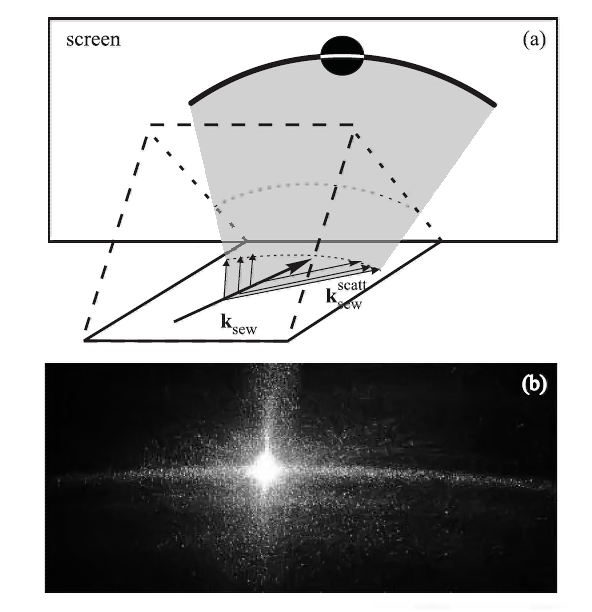
\includegraphics[scale=0.3]{gh3}
\end{center}

\column{6.5cm} 
Особенности эксперимента:

\begin{enumerate}

\item В отличие от поверхностного плазмон-поляритона ПЭФ возбуждаются s-падающей волной.
    Результат 16 мкм ($30 \lambda$), это почти в 10 раз больший сдвиг, чем без ФК!

\item Длина волны: 532 нм, мощность 10 мВт, угловая расходимость 2.5 мрад, размер пятна на ФК около 50 мкм, микроскоп $NA = 0.28$

\item Изменяя период ФК мы можем изменять длины волны ПЭВ.
\end{enumerate}

\end{columns}
Наблюдать поверхностную электромагнитную волну в дальней зоне невозможно. Но
благодаря шероховатостям поверхности брэгговского зеркала (одномерного фотонного кристалла) можно
наблюдать рассеянное излучение от ПЭВ, указывающее косвенно на ее существование.

\end{frame}


\begin{frame}{Усиление сдвига Гуса-Хенхен на фотонном кристалле}

 научная группа А.А. Федянина, МГУ
\begin{columns}[c]
\column{2.0in}
\begin{center}
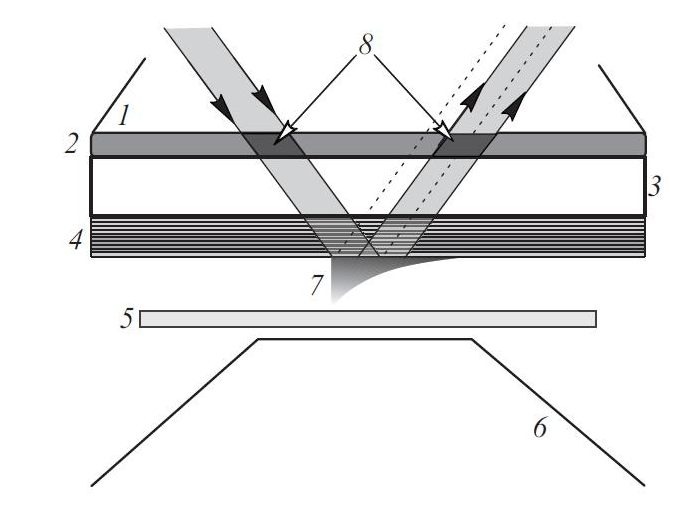
\includegraphics[scale=0.3]{gh4a}
\end{center}
\column{2.0in}
\begin{center}
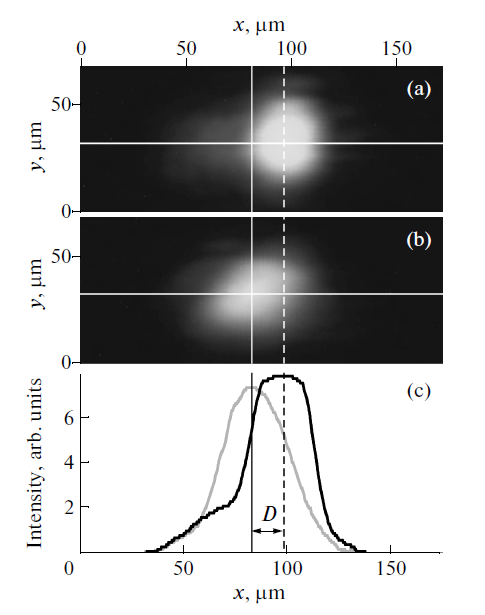
\includegraphics[scale=0.35]{gh4}
\end{center}


\end{columns}

\end{frame}






\end{document}








